
% First introduce what we've done
% Show cycles pie chart and tell why we put our focus on the four fat parts
In this section, we will fist briefly explain the baseline implementation of the LARS algorithm.
We also state the assumption that simplify the code. 
We then elaborate on how we optimize the most time-consuming parts of the algorithm and go through some general optimization.


% \subsection{Baseline implementation}
% General overview on baseline implementation
% Assumptions
% How we segment our code and why

Since each step of the algorithm requires results from the previous step, we segmented our code into several segments as mentioned in Table~\ref{tab:cost}.

The baseline is a straight-forward implementation of Algorithm~\ref{alg:lars} in C++ from scratch. The dictionary $X$, the largest array of the algorithm, is store in a column-majored format before any optimization. For implementation simplicity, we assume both dimensions of the dictionary, $d$ and $k$, are power of two and divisible by 16. Figure~\ref{fig:pie_before} shows that \textsc{Compute\_Lambda}, \textsc{Compute\_A}, and \textsc{Cholesky} are the most expensive components. So optimizing these parts has the highest priority. 

\begin{figure}
\centering
  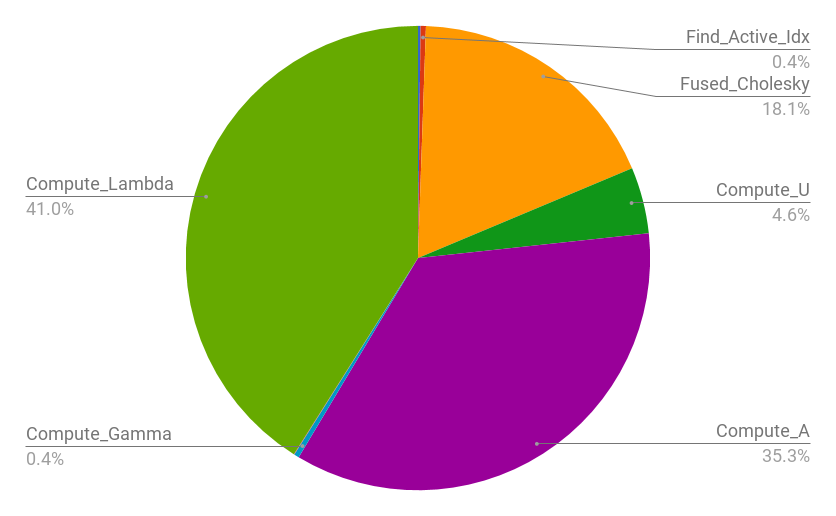
\includegraphics[scale=0.29]{./pic/pie_before.png}
  \caption{Run time before optimization}
  \label{fig:pie_before}
\end{figure}

\subsection{Reuse previous computation}
Most part of our algorithm is computational bounded. Therefore, we try to find redundant computations and reuse the result of previous computation if possible.
Possible methods proposed are storing previous computed value and reuse previous computation according to mathematical implications.

\mypar{Trade computation with memory}
In the beginning of each iteration, LARS check if the current approximation hit the regularize parameter $\lambda$. The equation used to compute $\lambda$ is shown in line~\ref{alg:lars:compute_lambda} in Algorithm~\ref{alg:lars}.
It is clear that 
\begin{equation}
    \begin{split}
        \Lambda &= X_A^T ( X_A \hat{\beta} - y) \\
                &= X_A^T X_A \hat{\beta} - X_A^T y \\
                &= G_A \hat{\beta} - X_A^T y
    \end{split}
\end{equation}
Since $G_A$ is calculated when updating the Cholesky solver in line~\ref{alg:lars:cholesky} of Algorithm~\ref{alg:lars}, we store this value in a new variable $G_A$. This requires more memory for variables since previously solving an incremental Cholesky system only need the last row in each iteration.
Since this method not only save computation time but also reduce accessed memory, which is $\mathbb{R}^{|A| \times |A|}$ now while the previous one is $\mathbb{R}^{|A| \times k}$, where $|A|$ is the size of the active set, we achieve significant speed-up in this segment after this modification.

\mypar{Remove computation using mathematical implication}
In the original baseline version of the algorithm, the target value $s_A$ fed into the Cholesky solver is re-computed at every iteration (line~\ref{alg:lars:get_active_idx_end}, Algorithm~\ref{alg:lars}), because the correlation between the current residual and the target is updated according to the current approximation in each iteration (line~\ref{alg:lars:get_active_idx}, Algorithm~\ref{alg:lars}).
Since the algorithm assures convergence, it shows that the sign of the correlation does not change once it is added into the active set.
Therefore, instead of recomputing the sign of each entry in every iteration, only the sign of the latest added entry is calculated in each iteration.

\subsection{Improve locality}
Since there are a lot of memory access throughout the algorithm.
We proposed several effective methods to take advantage of CPU caching.

\mypar{Compress stored data}
To keep track of the Cholesky decomposition of the correlation matrix $G$, we record the lower triangular matrix $L$, where $G = LL^T$. Since all the entries of $L$ above the main diagonal are zero and never used, instead of storing $L$ as a square matrix, we store only the lower triangle as a flattened one dimensional array. Even though in this case we lose much data alignment, it turns out to bring more benefits by fitting more of $L$ into cache.

The gram matrix $G_A$ also appears in the optimized version for computing $\lambda$ in the beginning of each iteration. Instead of storing the entire gram matrix, we only stored the lower triangular matrix using the compressed form.

\mypar{Switch to column orientation for $L^T$}
The Cholesky updating step solves a system of $L$ while the Cholesky inverting step solves a system of L and then a system of $L^T$. To solve two systems of $L$ and one of $L^T$, the program needs to go through every entry in $L$ three times. We don't store $L^T$ explicitly. Instead, while solving a system of $L^T$, the program accesses $L$ in the required order. As a Gaussian elimination can be conducted in either row orientation or column orientation, we pick the proper orientation for the system of $L$ and the system of $L^T$ respectively. 

\mypar{Fuse $L$ solving}
Furthermore, we fuse the Cholesky updating step with the Cholesky inverting step for both of them are solving a system of $L$. We can solve the system with different right-hand sides simultaneously. This way we only need to go through $L$ twice, one for the systems of $L$ and the other for the system of $L^T$.

\begin{figure}
\begin{subfigure}{.23\textwidth}
  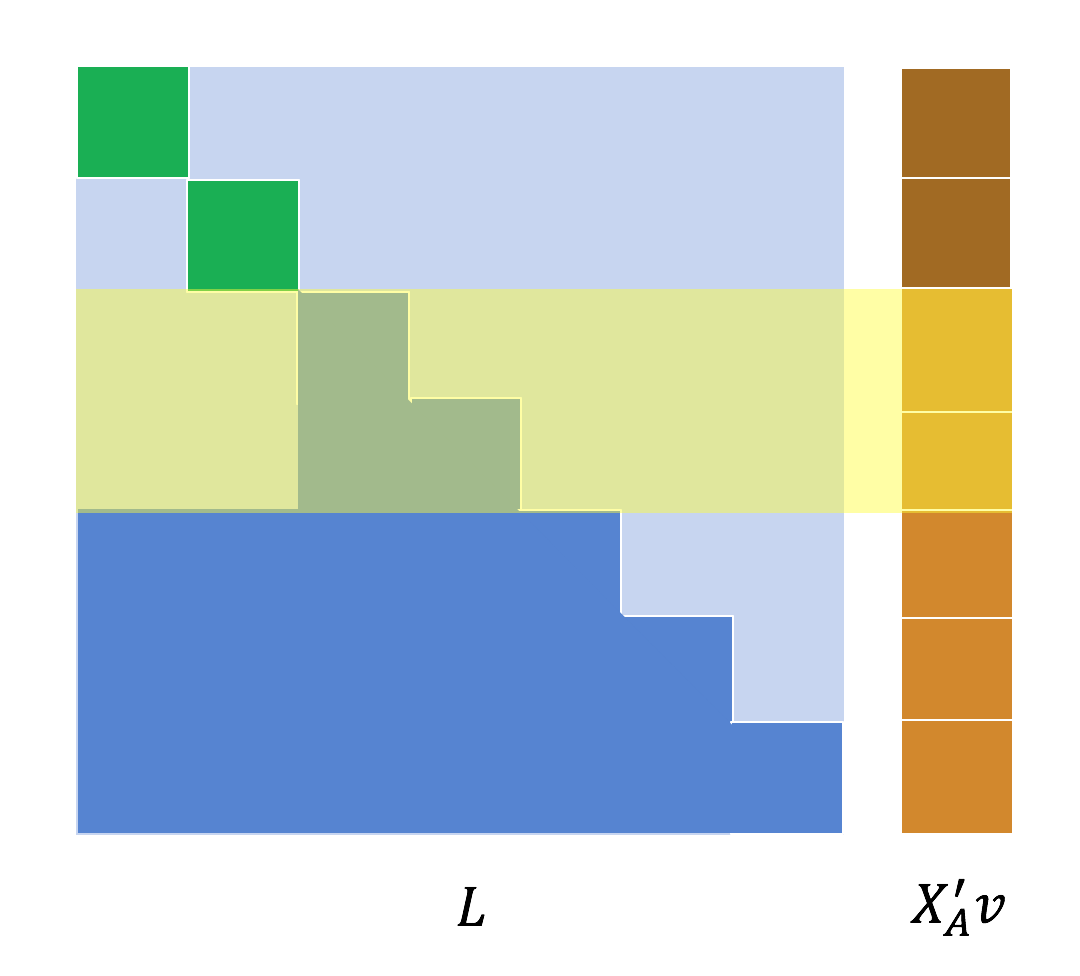
\includegraphics[scale=0.2]{./pic/block_cholesky.png}
  \caption{Block triangular solve}
  \label{fig:block_cholesky}
\end{subfigure}%
\begin{subfigure}{.22\textwidth}
  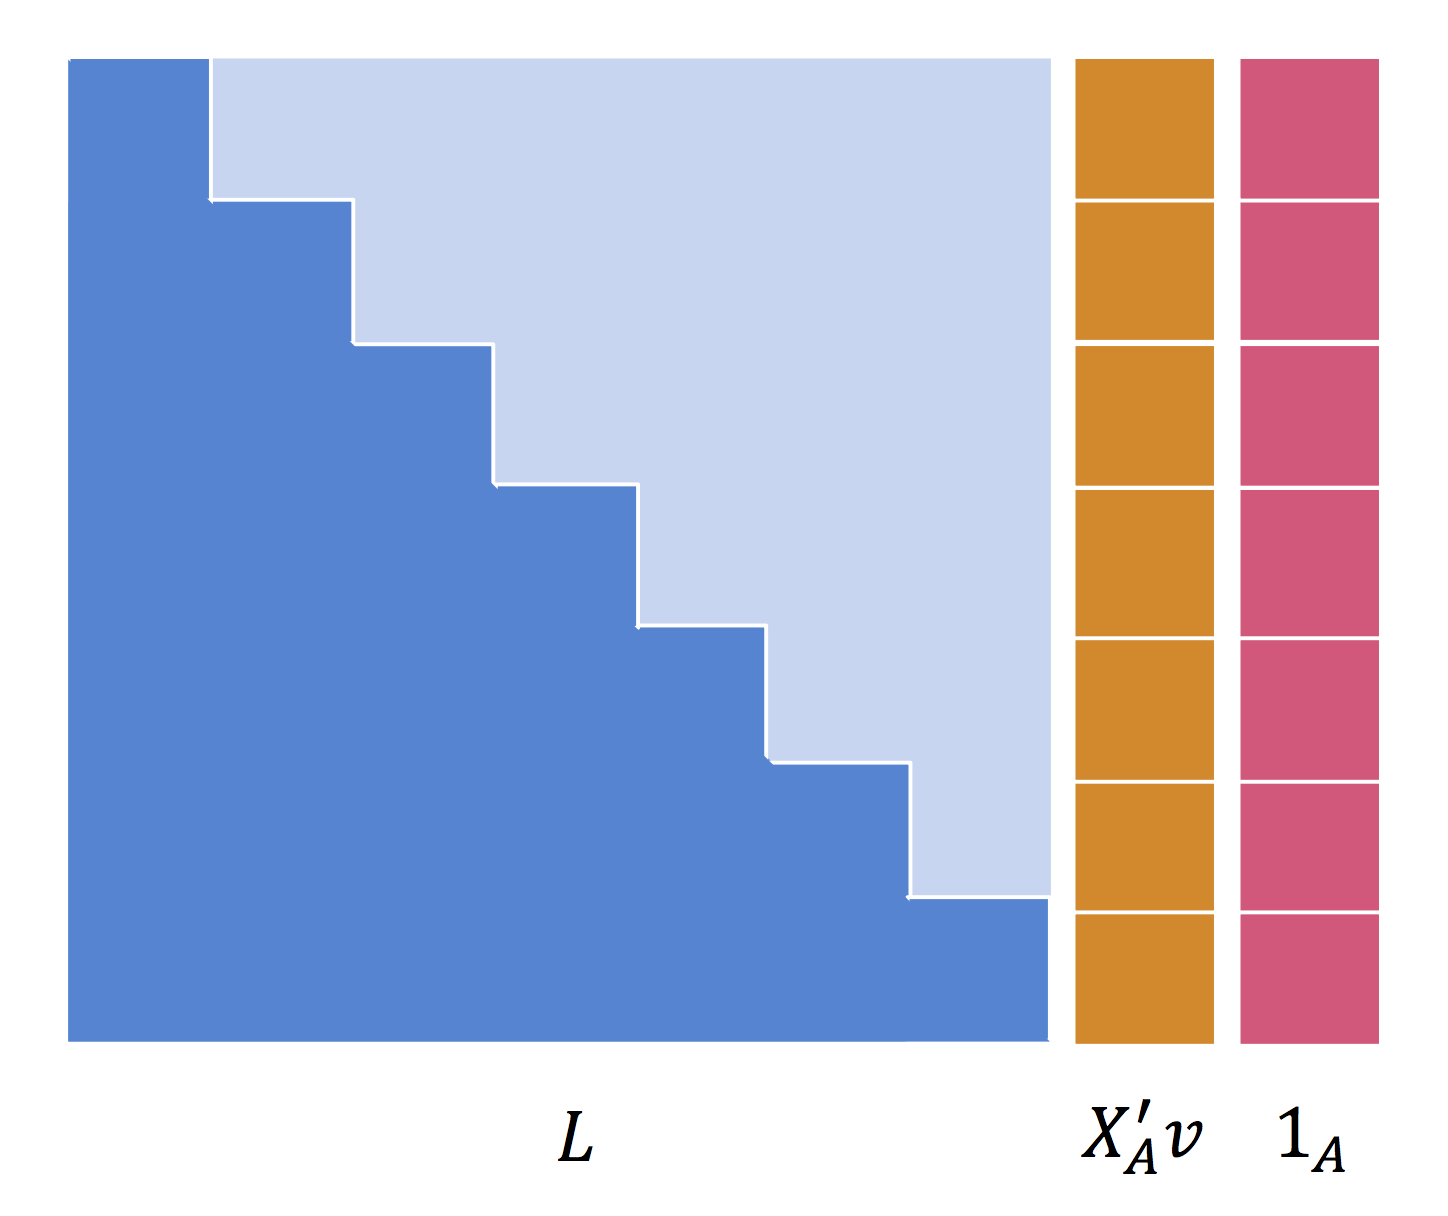
\includegraphics[scale=0.155]{./pic/fuse_cholesky.png}
  \caption{Fused triangular solve}
  \label{fig:fuse_cholesky}
\end{subfigure}
\caption{Optimization of Cholesky decomposition}
\label{fig:test}
\end{figure}

While reusing the value of the gram matrix $G_A$ to compute $\lambda$, both the lower triangular matrix of $G_A$ and its transpose are needed for computation: $G_A \hat{\beta} = L_{G_A} L_{G_A}^T \hat{\beta}$. We fuse the two multiplication by accessing each entry of $L_{G_A}$, the lower triangular matrix of $G_A$, only once.

\mypar{Blocking} All calculations done on the triangular solver in Cholesky is blocked with block size 128, so that each block fits in the L2 cache. 
Similarly, when computing $u_A$ and $a$ (line~\ref{alg:lars:get_u} and line~\ref{alg:lars:get_a} in Algorithm~\ref{alg:lars}), the matrices and vectors are also blocked to size 512 to improve locality.
Computing $\lambda$ (line~\ref{alg:lars:compute_lambda} in Algorithm~\ref{alg:lars}) is also blocked and is set to a block size of 16 after several testings on the optimal block size.


% compute vector A, access X in order
\mypar{Access large data structure in order}
Since $X_A$ is only a permuted subset of columns in $X$, we does not really record every entry in $X_A$. Instead, we only record the order of the number of column in $X$ that is added into $X_A$ in our baseline version.

To get the direction to move on, it is necessary to compute $u_A = A_A X_A w_A$ and $a = X^T u_A$, as shown in line~\ref{alg:lars:get_u} in Algorithm~\ref{alg:lars}.
The problem here is that to access $X_A$ in order, we will be jumping from rows to rows in $X$.
Since $X$ is large, it might cause multiple larger level cache misses.

To prevent this from happening, the best way is to sort the active set $A$ so that you access everything throughout the algorithm in order.
However, since we use incremental cholesky in our algorithm, we could not directly sort the active set in every iteration.
Therefore, we only attempt to access large data chunk, $X$, in order, while accessing smaller component $u_A$ incontinuously.

\subsection{Instruction-level parallelism and vectorization}
After improving the locality we vectorize most of our code with Intel X86 AVX2 intrinsics.
With the specific operations provided by the library, we are able to indicate FMA operations,
unroll for loops and remove if branches.

\mypar{unroll and scalar replacement}
To avoid blocking and increase instruction-level parallelism, we also implemented unrolling plus scalar replacement in for loops.
We also tested unrolling in each segment of the code until we get the best unrolling factor.

\mypar{remove if branches}
To calculate the absolute value, the sign value, checking whether a column is already activated and getting only values that satisfy some constraints create expensive if branches throughout the algorithm.
We therefore replace these if branches by combining \texttt{blendv} and \texttt{cmp} to get rid of the overhead caused by if branches.







% Now comes the ``beef'' of the paper, where you explain what you
% did. Again, organize it in paragraphs with titles. As in every section
% you start with a very brief overview of the section.

% For this class, explain all the optimizations you performed. This mean, you first very briefly
% explain the baseline implementation, then go through locality and other optimizations, 
% and finally SSE (every project will be slightly different of course). Show or mention 
% relevant analysis or assumptions. A few examples: 1) Profiling may lead you to 
% optimize one part first; 2) bandwidth plus data transfer analysis may show that 
% it is memory bound; 3) it may be too hard to implement the algorithm in full 
% generality: make assumptions and state them (e.g., we assume $n$ is divisible 
% by 4; or, we consider only one type of input image); 4) explain how certain data 
% accesses have poor locality. Generally, any type of analysis adds value to your work.

% As important as the final results is to show that you took a structured, organized 
% approach to the optimization and that you explain why you did what you did.

% Mention and cite any external resources including library or other code.

% Good visuals or even brief code snippets to illustrate what you did are good. 
% Pasting large amounts of code to fill the space is not good.

